\seclab{Discussion}{disco}
As seen in \secref{results}, the Lasso solution tends to minimize the error by truncating a lot of weights at 0 hence making it a sparse solution. Considering the fact that it actually prefers solutions where it solely predicts ages close to the mean age of the data sets, it is evident that the model has low variance and high bias. Actually the solution is too sparse since it does not allow for predictions in the outer regions of the age-spectrum of the data. Hence, even though we can collect some valuable knowledge from the Lasso regression it would be nice to create a model which allows for more variance in its predictions. 
To alleviate the pain of too little variance, we discussed if sequential feature selection (i.e. forward selection) could do the trick. In forward selection, one starts by creating all possible linear models with only 1 eigenface. Then the eigenface which alone gives the lowest value to the chosen dissimilarity measure will be added to the final feature list. Afterwards new linear models are trained with the first chosen eigenface \textit{and} a new eigenface where all possibilities are addressed again, choosing the next feature, i.e., the one that minimizes the dissimilarity measure the most. This procedure is continued until the chosen dissimilarity measure cannot be reduced by adding another feature or reaching a preset feature limit. During the final stages of our project work, we had a chance to construct such a model. This should allow for weights with greater absolute value compared to those of the Lasso regression.

\subsection{Sequential Feature Selection - Forward Selection}

\subsubsection{Results of the Forwards selection model}

The dissimilarity measure chosen for the forward selection model was a MSE based on the results of a linear regression of the training data compared to the actual results of the test data. The test and training data was split using a 10-fold cross-validation. Running the forward selection model with the before-described dissimilarity measure, under the constraint that the maximum number of features to include is 16 (corresponding to the number of chosen eigenfaces for the men by the Lasso regression), we get a MSE of 137.0 for both male and female. This is of course a measure of the training error which is inherently smaller than that of the generalization error, which makes it hard to compare one-to-one. However, since the weights in general have a greater absolute value compared to that of the Lasso regression, one can claim that they allow for more variance and thus better predictions.

In \figref{M_fs} and \figref{F_fs} we see the results of the sequential feature selection model for the males and females respectively. The left pane in both images shows the 16 eigenfaces chosen by the forward selection whereas the right pane shows the linear variation in age. Interestingly many of the features commented upon in \secref{results} still hold (some of the eigenfaces are actually identical). Examples include the facial hair and glasses for the men, and the grainy images for the women.

Another interesting point arises from the fact that the variance in the linearly varying age for both the males and females seem to be higher in comparison to the Lasso results. This goes hand in hand with the statement that the sum of the weights is higher.

\begin{figure}[ht!]
    \centering
    \begin{minipage}{0.49\textwidth}
    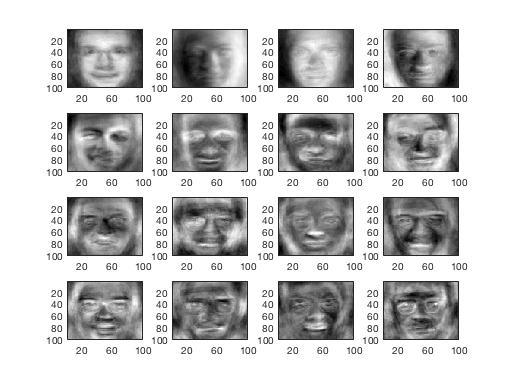
\includegraphics[width=1\linewidth]{fig/M_fs.png}
    \end{minipage}
    \begin{minipage}{0.49\textwidth}
    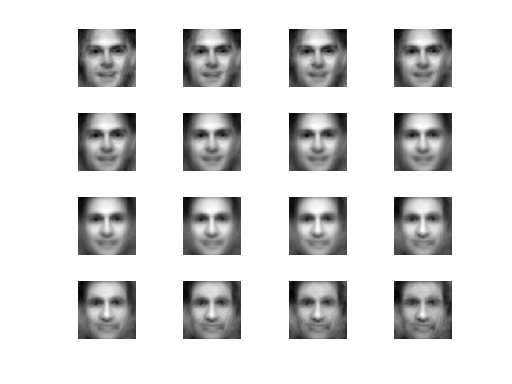
\includegraphics[width=1\linewidth]{fig/M_fs_Age.png}
    \end{minipage}
    \caption{Left: The chosen eigenfaces from the Forward Feature Selection ordered from the eigenface with the largest negative weight to the eigenface with the largest positive weight. Right: A linearly varying age based on the linear extension of the Forward Feature Selection linear model for males, from the mean age minus 30 years to the mean age plus 30 years.}
    \label{fig:M_fs}
\end{figure}

\begin{figure}[ht!]
    \centering
    \begin{minipage}{0.49\textwidth}
    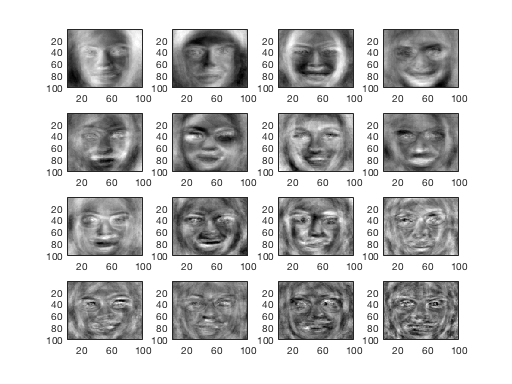
\includegraphics[width=1\linewidth]{fig/F_fs.png}
    \end{minipage}
    \begin{minipage}{0.49\textwidth}
    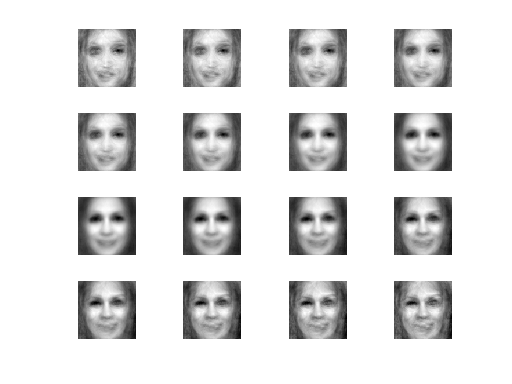
\includegraphics[width=1\linewidth]{fig/F_fs_Age.png}
    \end{minipage}
    \caption{Left: The chosen eigenfaces from the Forward Feature Selection ordered from the eigenface with the largest negative weight to the eigenface with the largest positive weight. Right: A linearly varying age based on the linear extension of the Forward Feature Selection linear model for females, from the mean age minus 30 years to the mean age plus 30 years.}
    \label{fig:F_fs}
\end{figure}

\subsection{Future prospects within the scope of this project}
Since the project phase of this course was \textit{"only"} 2.5 ECTS points of time, we have not had the time to go into detail with as many aspects of the project as we would have liked. Hence there are various parts of the project which could have benefited from additional work. Some of which will be discussed in this subsection.
\subsubsection{More appropriate dissimilarity measure for Lasso}
At the moment, we use the MSE as dissimilarity measure for choosing the right model in the Lasso regression model. However, other dissimilarity measures should be considered and an example of such a dissimilarity measure could be to count the number observations a given model fails to predict within a given range of a target. 

\subsubsection{A professional data-set}
Since the data used for our modelling is taken from an open database where the images are mainly taken by paparazzi or screen-shots from movies, the lighting of the images is not the same, photos are taken from different angles and the facial expressions vary a lot. Hence it would have been beneficial to create a professional data set made for such an experiment. It would have been beneficial to use a data set which did not contain familiar faces in the form of actors and actresses as this inevitably introduces some bias to how our subjects perceived age.